\documentclass[11pt]{article}
\usepackage[margin=0.75in]{geometry}
\usepackage{tikz}
\usepackage{amsmath}
\usepackage{amssymb}
\usepackage{xcolor}
\usepackage{enumitem}
\usetikzlibrary{arrows.meta, patterns}


\begin{document}

\begin{center}
    \textbf{In-class Tutorial: Fabry-P\'erot Dark Offset Transfer Function}\\
    March 16, 2026\\
    Lasers and Optomechanics\\~\\
    Name: \underline{\hspace{10cm}}
\end{center}


\vspace{0.2cm}



\noindent
\textbf{Sensing the Fabry-P\'erot's Resonance}\\
Suppose we have a Fabry-P\'erot interferometer.
We would like to know whether the Fabry-P\'erot is on resonance.
Here we will explore possibilities for sensing the resonance of a Fabry-P\'erot cavity,
especially in the presence of length disturbances $\Delta L(t)$.


\begin{center}
  
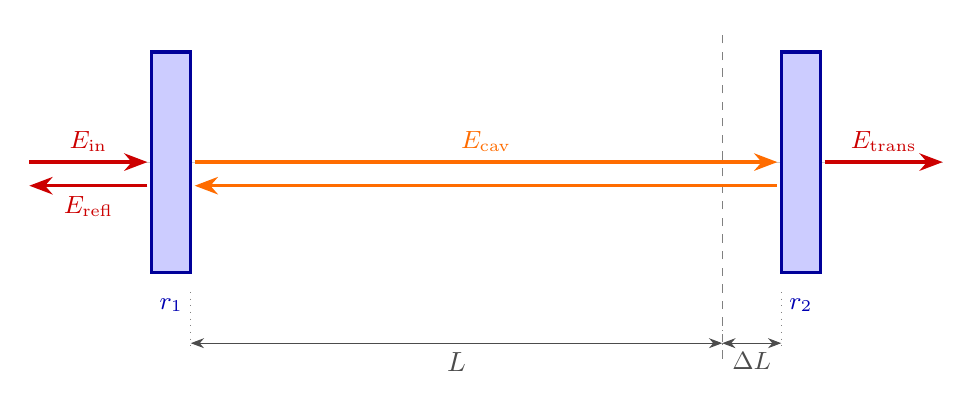
\begin{tikzpicture}[
    >=Stealth,
    thick,
    beam/.style={->, very thick, red!80!black},
]
 
%--- Coordinates ---
\def\Lx{0}        % input mirror center x
\def\Rx{7}        % nominal end mirror x (for label L)
\def\RxShift{8.0} % actual end mirror center x (moved back for Delta L space)
\def\mirH{1.4}    % half-height of mirrors
\def\mirW{0.25}   % half-width of mirror rectangles
\def\beamY{0}     % beam axis y
 
%--- Cavity axis (thin guide line) ---
\draw[gray!40, thin] (\Lx-1.8, \beamY) -- (\RxShift+1.8, \beamY);
 
%--- Input mirror rectangle (r1) ---
\filldraw[fill=blue!20!white, draw=blue!60!black, line width=1.2pt]
    (\Lx-\mirW, -\mirH) rectangle (\Lx+\mirW, \mirH);
\node[below, blue!70!black, font=\small] at (\Lx, -\mirH-0.2) {$r_1$};
% Minus sign on interior (right) face of r1
\node[font=\large, black] at (\Lx+\mirW+0.22, 0) {$-$};
 
%--- Nominal end mirror position (vertical dashed line only) ---
\draw[dashed, gray, thin] (\Rx, -\mirH-1.1) -- (\Rx, \mirH+0.3);
 
%--- Actual end mirror rectangle (r2), displaced by Delta L ---
\filldraw[fill=blue!20!white, draw=blue!60!black, line width=1.2pt]
    (\RxShift-\mirW, -\mirH) rectangle (\RxShift+\mirW, \mirH);
\node[below, blue!70!black, font=\small] at (\RxShift, -\mirH-0.2) {$r_2$};
% Minus sign on interior (left) face of r2
\node[font=\large, black] at (\RxShift-\mirW-0.22, 0) {$-$};
 
%--- Delta L annotation (dashed line to front face of end mirror) ---
\draw[<->, thin, black!70]
    (\Rx, -\mirH-0.9) -- (\RxShift-\mirW, -\mirH-0.9)
    node[midway, below, font=\small] {$\Delta L$};
\draw[dotted, thin, gray] (\Rx,           -\mirH-0.65) -- (\Rx,           -\mirH-1.0);
\draw[dotted, thin, gray] (\RxShift-\mirW, -\mirH-0.25) -- (\RxShift-\mirW, -\mirH-1.0);
 
%--- Cavity length label L (below cavity, same row as Delta L) ---
\draw[<->, thin, black!70]
    (\Lx+\mirW, -\mirH-0.9) -- (\Rx, -\mirH-0.9)
    node[midway, below] {$L$};
\draw[dotted, thin, gray] (\Lx+\mirW, -\mirH-0.25) -- (\Lx+\mirW, -\mirH-1.0);
 
%--- Input beam E_in (on axis, from left to mirror face) ---
\draw[beam] (-1.8, 0) -- (\Lx-\mirW-0.05, 0)
    node[midway, above, font=\small] {$E_\mathrm{in}$};
 
%--- Reflected beam E_refl (going back left, below axis) ---
\draw[beam] (\Lx-\mirW-0.05, -0.3) -- (-1.8, -0.3)
    node[midway, below, font=\small] {$E_\mathrm{refl}$};
 
%--- Intracavity beam E_cav: forward pass (on axis, same height as E_in) ---
\draw[beam, orange!85!red] (\Lx+\mirW+0.05, 0) -- (\RxShift-\mirW-0.05, 0)
    node[midway, above, font=\small] {$E_\mathrm{cav}$};
 
%--- Intracavity return pass (aligned with E_refl at y=-0.3) ---
\draw[beam, orange!85!red, <-]
    (\Lx+\mirW+0.05, -0.3) -- (\RxShift-\mirW-0.05, -0.3);
 
%--- Transmitted beam E_trans (on axis, exiting right) ---
\draw[beam] (\RxShift+\mirW+0.05, 0) -- (\RxShift+1.8, 0)
    node[midway, above, font=\small] {$E_\mathrm{trans}$};
 
\end{tikzpicture}
\end{center}

Above we have a diagram of a Fabry-P\'erot cavity, 
with a nominal length $L$, but also some static offset $\Delta L$.
We will explore our capability to monitor and restore our lock in the case of a static offset.

Recall that field transfer functions of the lossless Fabry-Perot were 
\begin{align}
\dfrac{E_\mathrm{refl}}{E_\mathrm{in}} = \dfrac{r_1 - r_2 e^{-i 2 \phi}}{1 - r_1 r_2 e^{-i 2 \phi}}, \qquad
\dfrac{E_\mathrm{cav}}{E_\mathrm{in}} = \dfrac{t_1}{1 - r_1 r_2 e^{-i 2 \phi}}, \qquad
\dfrac{E_\mathrm{trans}}{E_\mathrm{in}} = \dfrac{t_1 t_2 e^{-i \phi}}{1 - r_1 r_2 e^{-i 2 \phi}}
\end{align}

\noindent
\textbf{Part 1: Transmitted Power}\\
The easiest way to tell if light is resonating in the cavity is to look at the transmitted beam.
Intuitively, there is a maximum transmitted light when the light in the cavity is maximized.

\begin{enumerate}
    \item Derive an expression for the transmitted \textit{power} $P_\mathrm{trans}(\phi)$.
    \item What is the maximum transmitted power at resonance $P_\mathrm{trans}(0)$?
    \item Starting at resonance, what happens to the transmitted power when the cavity gets longer?
    \item Starting at resonance, what happens to the transmitted power when the cavity gets shorter?
    \item Would it be possible to use the transmitted power to \textit{restore} resonance in case of some disturbance $\Delta L$?  How might you try to go about it?
\end{enumerate}

\vspace{0.3cm}

\noindent
\textbf{Part 2: Reflected Power}\\
Another option we can analyze is the power in reflection of the cavity $P_\mathrm{refl}$:

\begin{enumerate}
    \item Derive an expression for the reflected power $P_\mathrm{refl}(\phi)$.  What is the reflected power at resonance?
    \item Set $r_2 = r_1 = r$.  Does $P_\mathrm{refl}(\phi)$ simplify at all?  What value do you get at resonance?
    \item Starting at resonance, what happens to the reflected power when the cavity gets longer? Shorter?
    \item Can you use reflected power to restore resonance?
\end{enumerate}



\noindent
\textbf{Part 3: Reflected Field}\\
From looking at the transmitted and reflected power, we cannot directly use the power signals from the interferometer to hold onto resonance.
But we have ignored a crucial signal coming from the interferometer, the phase.
Here we will calculate the change in reflected field $\dfrac{d E_\mathrm{refl}}{d \phi}$.

\begin{enumerate}
    \item Derive an expression for the change in reflected field with respect to phase $\phi$: $\dfrac{d E_\mathrm{refl}}{d\phi}(\phi)$.\\
    \textit{Answer: $\dfrac{d E_\mathrm{refl}}{d\phi}(\phi) = \dfrac{i 2 r_2 (1 - r_1^2) e^{-i 2 \phi}}{(1 - r_1 r_2 e^{-i 2 \phi})^2}$}
    \item Set $r_2 = r_1 = r$.  What is $E_\mathrm{refl}(0)$?  What is $\dfrac{d E_\mathrm{refl}}{d\phi}(0)$?
    \item What happens to the reflected field when the cavity gets longer? What about shorter?
    \item Could you use the reflected field to restore resonance?  What would you need in order to do so?
\end{enumerate}

\vspace{0.3cm}

\noindent
\textbf{Part 4: Dither Locking}\\
In Part 3, we found that it could be possible to use the reflected field phase.
But how may we measure this signal using photodetectors?

One solution is to introduce a modulation of the end mirror $\Delta x(t) \cos(\omega t)$.
By introducing a known length modulation of the intracavity field, 
we can ``rotate'' our phase signal into the amplitude quadrature, where it can be measured at the frequency $\omega$.

Below, we'll go through the math of how dither locking works for the reflected field.\\
The process is roughly:\\
A) Find the carrier's contribution to the reflected field (already done in Part 3).\\
B) Find the carrier field incident on the modulating mirror.\\
C) Create the audio sidebands.\\
D) Find the sidebands' contribution to the reflected field.\\
E) Find the total power signal $P_\mathrm{refl}(t)$.\\
F) Demodulate that power signal at $\omega$.\\
What we should find is a power signal at $\omega$ that is proportional to our static offset $\phi = k \Delta L$. 
If $\phi = 0$, our audio sideband fields should cancel exactly, giving us zero.
But if $\phi \neq 0$, we should get a power signal that changes sign at $\omega$,
which tells us which way to move our mirror to recover our resonance.


\begin{enumerate}
    \item First, find the transfer function from the end mirror $E_\mathrm{cav2}$ to the reflected field $E_\mathrm{refl}$.\\
    \textit{Answer: $\dfrac{E_\mathrm{refl}}{E_\mathrm{cav2}}(\phi) = \dfrac{t_1 e^{-i \phi}}{1 - r_1 r_2 e^{-i 2 \phi}}$}
    \item Find the carrier field incident on the end mirror $M_2$.
    \item Apply the length modulation $\Delta x(t) \cos(\omega t)$ to find the total field immediately reflected off the end mirror $E_\mathrm{cav2}$.  
    \textit{Hint: There should be three fields.}
    \item Apply your transfer function $\dfrac{E_\mathrm{refl}}{E_\mathrm{cav2}}(\phi)$ from (1) to your total $E_\mathrm{cav2}$ from (3) to find the total reflected field.  
    \textit{Hint: It may be easier to consider the accrued phases for carrier $\phi$ and for the audio sidebands $\phi \pm \eta$, where $\phi = \omega_0 L / c$ and $\eta = \omega L / c$.}
    \item Calculate the total reflected power $P_\mathrm{refl}(t)$.  Let $\Delta x^2 \rightarrow 0$ for small length modulations.
    \item Demodulate the total reflected power at $\omega$ to calculate $P^I_\mathrm{refl}$ and $P^Q_\mathrm{refl}$.  
\end{enumerate}


\end{document}